\documentclass[table,usenames,dvipsnames]{beamer}

\usepackage[english]{babel}
\usepackage[utf8]{inputenc}
\usepackage{listings}
\usepackage{datetime}
\usepackage{graphics}
\usepackage{fancybox}
\usepackage{color}
\usepackage[normalem]{ulem}
\usepackage{tikz}
\usepackage{verbatim}
\usetikzlibrary{shapes,arrows}
\usetheme{CambridgeUS}
\usecolortheme{seagull}
% Changing of bullet foreground color not possible if {itemize item}[ball]
\DefineNamedColor{named}{Purple}{cmyk}{0.52,0.97,0,0.55}
\setbeamertemplate{itemize item}[triangle]
\setbeamercolor{title}{fg=Purple}
\setbeamercolor{frametitle}{fg=Purple}
\setbeamercolor{itemize item}{fg=Purple}
\setbeamercolor{section number projected}{bg=Purple,fg=white}
\setbeamercolor{subsection number projected}{bg=Purple}

\renewcommand{\dateseparator}{.}
\newcommand{\todayiso}{\twodigit\day \dateseparator \twodigit\month \dateseparator \the\year}
\newcommand{\shell}[1]{\texttt{#1}}
\definecolor{LightGray}{gray}{0.9}

\title{Osnove korištenja operacijskog sustava Linux}
\subtitle{10. Ljuske}
\author[Goran Cetušić]{Goran Cetušić\\{\small Nositelj: dr. sc. Stjepan Groš}}
\institute[FER]{Sveučilište u Zagrebu \\
				Fakultet elektrotehnike i računarstva}
				
\date{\todayiso}

\begin{document}
    %\beamerdefaultoverlayspecification{<+->}
{
\setbeamertemplate{headline}[] % still there but empty
\setbeamertemplate{footline}{}

\begin{frame}
\maketitle
\end{frame}
}

\begin{frame}
\frametitle{Sadržaj}
\tableofcontents
\end{frame}

\section{Pojam ljuske}
\begin{frame}[t]
\frametitle{Pojam ljuske (1)}
\begin{itemize}
  \item Ljuska je program
  \item Služi za lakšu komunikaciju sa jezgrom
  \begin{itemize}
    \item Pokreće procese za korisnike
    \item Brine se za preusmjeravanje ulaza i izlaza
    \item Moguća je automatizacija naredbi
    \item \ldots
  \end{itemize}
  \item Sve zadatke je moguće obaviti pomoću ljuske
\end{itemize}
\end{frame}

\begin{frame}[t]
\frametitle{Pojam ljuske (2)}
\begin{itemize}
  \item Primjer
  \begin{itemize}
    \item Pokretanje procesa
  \end{itemize}
  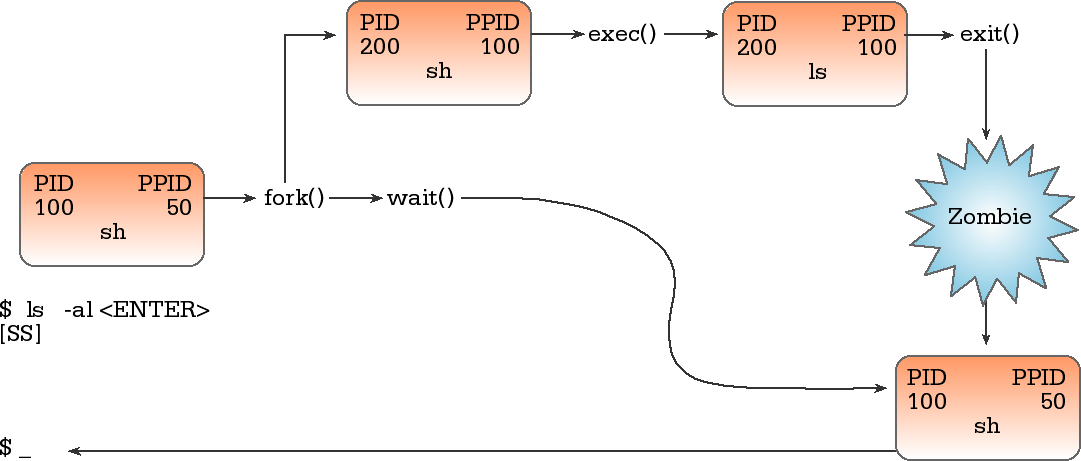
\includegraphics[width=\linewidth]{process_start}
\end{itemize}
\end{frame}

\begin{frame}[t]
\frametitle{Pojam ljuske (3)}
\begin{itemize}
  \item Nakon pokretanja terminala pokrenuta je ljuska sa izlazom i ulazom 
        vezanim za terminal
  \item Zadane naredbe interpretira ljuska, ne terminal
  \begin{tabular}{c c}
    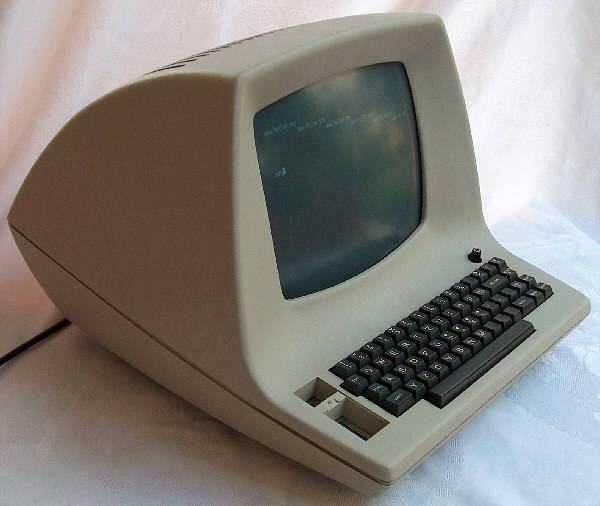
\includegraphics[width=0.45\linewidth]{terminal_old} &
    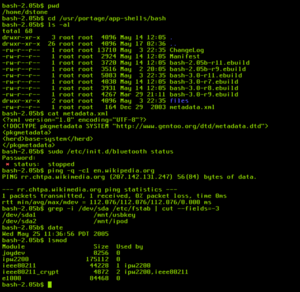
\includegraphics[width=0.45\linewidth,height=0.5\textheight]{terminal_new}
  \end{tabular}
\end{itemize}
\end{frame}

\begin{frame}[t]
\frametitle{Vrste ljuski}
\begin{itemize}
  \item Postoji nekoliko implementacija ljuski
  \begin{itemize}
    \item sh, bash, csh, ksh, \ldots
  \end{itemize}
  \item Korisnik ima izbor koju će koristiti
  \begin{itemize}
    \item Naredba \shell{chsh} mijenja ljusku korisnika
    \item Podatak o ljusci korisnika zapisan je u datoteci \shell{/etc/passwd} 
  \end{itemize}
  \item Popis dostupnih ljuski nalazi se u datoteci \shell{/etc/shells}
\end{itemize}
\end{frame}

\begin{frame}[t]
\frametitle{Bash ljuska}
\begin{itemize}
  \item Najkorištenija ljuska na Linux sustavu je \shell{bash} -- 
        \emph{Bourne again shell}
  \begin{itemize}
    \item Nasljednik \shell{sh} ljuske (\emph{Bourne shell}) i 
      kompatibilna s njom -- skripte pisane u \shell{sh} mogu biti 
      pokretane s \shell{bash} ljuskom, ali ne i obratno
    \item Neka dodatna svojstva
    \begin{itemize}
      \item Upravljanje poslovima (\shell{jobs}, \shell{bg}, \shell{fg})
      \item Neograničena povijest naredbi
      \item Pseudonimi (\emph{alias})
    \end{itemize}
  \end{itemize}
\end{itemize}
\end{frame}

\section{Varijable okruženja}
\begin{frame}[t]
\frametitle{Varijable okruženja (1)}
\begin{itemize}
  \item engl. \emph{environment variables}
  \item Slične varijablama u programskim jezicima
  \begin{itemize}
    \item Spremaju vrijednosti u varijable koje ostali programi ili sama 
          ljuska mogu čitati
  \end{itemize}
  \item Naredba \shell{env} izlistava varijable okruženja trenutne ljuske
  \item Zadatak
  \begin{itemize}
    \item Izlistajte varijable okruženja
  \end{itemize}
\end{itemize}
\end{frame}

\begin{frame}[t]
\frametitle{Varijable okruženja (2)}
\begin{itemize}
  \item Vrijednost varijable dohvaća se dodavanjem \shell{\$} ispred imena 
        varijable
  \item Primjer
  \begin{itemize}
    \item[] \shell{\$ echo PATH}
    \item[] \shell{PATH}
    \item[] \shell{\$ echo \$PATH}
    \item[] \shell{/usr/local/bin:/usr/bin:/bin:/usr/games}
  \end{itemize}
\end{itemize}
\end{frame}

\begin{frame}[t]
\frametitle{Bitnije varijable (1)}
\begin{itemize}
  \item \shell{PATH}
  \begin{itemize}
    \item Popis direktorija koji sadrže naredbe
    \item Zbog ove varijable možemo upisati ime naredbe bez navođenja 
          apsolutne staze
    \item Postavljena u jednoj od skripti kod pokretanja ljuske
  \end{itemize}
  \item Zadatak
  \begin{itemize}
    \item Ispisati varijablu \shell{PATH}
    \item Dodati direktorij \shell{/opt} varijabli \shell{PATH}
  \end{itemize}
\end{itemize}
\end{frame}

\begin{frame}[t]
\frametitle{Bitnije varijable (2)}
\begin{itemize}
  \item \shell{SHELL}
  \begin{itemize}
    \item Trenutna ljuska korisnika
  \end{itemize}
  \item \shell{HOME}
  \begin{itemize}
    \item Informacija koji je direktorij matični direktorij trenutnog 
          korisnika
    \item Moguće je koristiti skraćenice poput \shell{\~{}} 
  \end{itemize}
  \item Zadatak
  \begin{itemize}
    \item Što ispisuje \shell{ls -l \~{}}
  \end{itemize}
\end{itemize}
\end{frame}

\begin{frame}[t]
\frametitle{Postavljanje varijabli (1)}
\begin{itemize}
  \item Varijabla je postavljena dodjeljivanje vrijednosti
  \begin{itemize}
    \item Praksa je da se nazivi varijabli sastoje od velikih slova
  \end{itemize}
  \item Primjer
  \begin{itemize}
    \item[] \shell{\$ echo \$OKOSL}
    \item[] 
    \item[] \shell{\$ OKOSL=A102}
    \item[] \shell{\$ echo \$OKOSL}
    \item[] \shell{A102}
  \end{itemize}
\end{itemize}
\end{frame}

\begin{frame}[t]
\frametitle{Postavljanje varijabli (2)}
\begin{itemize}
  \item Ako otvorimo novu ljusku, varijabla neće biti postavljena
  \begin{itemize}
    \item Ako želimo da sve novopokrenute podljuske imaju postavljene neku
      varijablu, koristimo \shell{export}
    \item Samo podljuske mogu naslijediti varijable
  \end{itemize}
  \item Brisanje varijable ostvaruje se naredbom \shell{unset}
\end{itemize}
\end{frame}

\begin{frame}[t]
\frametitle{Postavljanje varijabli (3)}
\begin{itemize}
  \item Zadatak
  \begin{itemize}
    \item Osigurati da je varijabla \shell{OKOSL} postavljena
    \item Otvoriti podljusku trenutne ljuske
    \item Ispisati varijablu \shell{OKOSL}
    \item Izaći iz podljuske
    \item Izvršiti \shell{export OKOSL}
    \item Pokrenuti podljusku i ispisati varijablu \shell{OKOSL}
    \item Pokrenuti podljusku podljuske, ispisati varijablu \shell{OKOSL}
  \end{itemize}
\end{itemize}
\end{frame}

\section{Načini rada ljuske}
\begin{frame}[t]
\frametitle{Načini rada}
\begin{itemize}
  \item Bash ljusku je moguće pokrenuti na različite načine
  \begin{itemize}
    \item Interaktivno bez prijave
    \item Interaktivno sa prijavom
    \item Neinteraktivno
    \item Preko \shell{sh} naredbe
  \end{itemize}
  \item Svaki način utječe na ponašanje ljuske
\end{itemize}
\end{frame}

\begin{frame}[t]
\frametitle{Interaktivni način rada (1)}
\begin{itemize}
  \item Korisnik može unositi naredbe
  \item Ako se korisnik pri pokretanju ljuske prijavio (unio lozinku i 
        korisničko ime), ljuska izvršava datoteke
  \begin{itemize}
    \item \shell{/etc/profile}
    \item \shell{\~{}/.bash\_profile},\shell{\~{}/.bash\_login} ili 
          \shell{\~{}/.profile}
    \begin{itemize}
      \item pročitana je prva datoteka koja postoji
    \end{itemize}
    \item \shell{\~{}/.bash\_logout}
  \end{itemize}
\end{itemize}
\end{frame}

\begin{frame}[t]
\frametitle{Interaktivni način rada (2)}
\begin{itemize}
  \item Ako se korisnik pri pokretanju ljuske nije prijavio (unio lozinku i
        korisničko ime) ljuska izvršava datoteke
  \begin{itemize}
    \item \shell{\~{}/.bashrc}
    \item \shell{/etc/bash.bashrc}
    \begin{itemize}
      \item \shell{bashrc} je obično pozivana u \shell{bash\_profile}
      \item[] \shell{if [ -f \~{}/.bashrc ]; then . \~{}/.bashrc; fi}
    \end{itemize}
  \end{itemize}
  \item Zadatak
  \begin{itemize}
    \item Ispisati varijablu \shell{-}
  \end{itemize}
\end{itemize}
\end{frame}

\section{Skripte}
\begin{frame}[t]
\frametitle{Skripte (1)}
\begin{itemize}
  \item Skripte služe za izvršavanje skupa naredbi
  \begin{itemize}
    \item Izvršena skripta napravit će sve kao da je utipkano u terminal
    \item Rade u neinteraktivnom modu
    \item Ne čitaju iste skripte kao interaktivni mod
    \begin{itemize}
      \item Čitaju skripte navedene u varijabli \shell{BASH\_ENV}
    \end{itemize}
  \end{itemize}
  \item Bash nije samo ljuska već i skriptni jezik (vidljivo po navedenoj 
        if konstrukciji)
\end{itemize}
\end{frame}

\begin{frame}[t]
\frametitle{Skripte (2)}
\begin{itemize}
  \item Postoji mnoštvo vrsta skripti
  \begin{itemize}
    \item Python, Perl, Bash, PHP, \ldots
  \end{itemize}
  \item Prva linija određuje koja naredba će interpretirati skriptu
  \item Za Bash skriptu to je
  \begin{itemize}
    \item[] \shell{\#! /bin/bash}
    \item \shell{\#!} znači da slijedi lokacija programa koji će 
          interpretirati skriptu (s ili bez razmaka)
  \end{itemize}
\end{itemize}
\end{frame}

\begin{frame}[t]
\frametitle{Skripte (3)}
\begin{itemize}
  \item Skripte NISU interaktivne
  \begin{itemize}
    \item Mogu izvršiti samo predefinirani skup naredbi
  \end{itemize}
  \item Skripta mora imati dopuštenja da bude izvršena
  \item Ako direktorij u kojem se nalazi nije u \shell{PATH} varijabli, 
        mora se navesti puna staza
  \item Zadatak
  \begin{itemize}
    \item Napisati Bash skriptu koja ispisuje ``Hello World!''
    \item Izvršiti skriptu
  \end{itemize}
\end{itemize}
\end{frame}

\begin{frame}[t]
\frametitle{Skripte (4)}
\begin{itemize}
  \item Pokrenuta skripta stvori podljusku, izvrši naredbe i vrati se u 
        izvornu ljusku
  \begin{itemize}
    \item Korisno ako želimo podesiti okruženje nove ljuske
    \item Može stvoriti probleme ako skripta pretpostavlja okruženje 
          trenutne ljuske
  \end{itemize}
  \item Ako želimo da se skripta izvrši u trenutnoj ljusci, koristimo 
        \shell{source} ili \shell{.} (točka)
\end{itemize}
\end{frame}

\begin{frame}[t]
\frametitle{Skripte (5)}
\begin{itemize}
  \item Zadatak
  \begin{itemize}
    \item Dodati varijablu \shell{OKOSL} prethodnoj skripti
    \item[] \shell{export OKOSL=A102}
    \item Izvršiti skriptu
    \item Izvršiti ponovno u trenutnoj ljusci
    \item Svaki put ispisati OKOSL
    \item Što se dogodilo kod drugog ispisa i zašto?
    \item Je li se promjena propagirala na ljusku roditelja korištenjem 
          \shell{export}?
  \end{itemize}
\end{itemize}
\end{frame}

\section{Povijest naredbi}
\begin{frame}[t]
\frametitle{Nadopunjavanje naredbi}
\begin{itemize}
  \item Bash omogućava brže pisanje naredbi njihovim nadopunjavanjem unutar
        komandne linije
  \begin{itemize}
    \item Pretražuje naredbe i korisniku ponudi jednu od mogućnosti na 
          temelju dosadašnjeg unosa znakova
  \end{itemize}
  \item Koristi se tipka TAB
  \begin{itemize}
    \item Jedan TAB nadopunit će naredbu ako postoji samo jedna mogućnost
    \item Dvaput TAB će korisniku ispisati sve mogućnosti
  \end{itemize}
\end{itemize}
\end{frame}

\begin{frame}[t]
\frametitle{Povijest naredbi (1)}
\begin{itemize}
  \item Datoteka \shell{\~{}/.bash\_history} sadrži popis svih naredbi koje
        su izvršene
  \begin{itemize}
    \item Nove naredbe su zapisane tek nakon terminiranja ljuske
    \item Ljuska učita povijest naredbi tijekom pokretanja
    \item Dvije ljuske nemaju istu povijest naredbi ako su korištene 
          konkurentno, ali nakon ponovno pokretanja obiju ljusaka, povijest
          je ista
  \end{itemize}
\end{itemize}
\end{frame}

\begin{frame}[t]
\frametitle{Povijest naredbi (2)}
\begin{itemize}
  \item Zadatak
  \begin{itemize}
    \item Pokrenuti istovremeno dvije zasebne ljuske
    \item Pročitati zadnju naredbu u \shell{\~{}/.bash\_history}
    \item Upisati različite naredbe u ljuske
    \item Pročitati zadnju naredbu u \shell{\~{}/.bash\_history}
    \item Terminirati jednu ljusku
    \item Pročitati zadnju naredbu u \shell{\~{}/.bash\_history}
    \item Terminirati drugu ljusku
    \item Pročitati zadnju naredbu u \shell{\~{}/.bash\_history}
  \end{itemize}
\end{itemize}
\end{frame}

\begin{frame}[t]
\frametitle{Povijest naredbi (3)}
\begin{itemize}
  \item Za izvršavanje posljednje korištene naredbe koristi se \shell{!!}
  \begin{itemize}
    \item Isto tako \shell{!<znakovi>} će izvršiti posljednju naredbu koja
          je tog oblika npr. \shell{!ssh}
  \end{itemize}
  \item Primjer
  \begin{itemize}
    \item[] \shell{\$ cat /etc/shadow}
    \item[] \shell{cat: /etc/shadow: Permission denied}
    \item[] \shell{\$ sudo !!}
  \end{itemize}
\end{itemize}
\end{frame}
      
\begin{frame}[t]
\frametitle{Pretraživanje povijesti naredbi}
\begin{itemize}
  \item Što ako znamo otprilike kako je glasila naredba ali se ne možemo 
        sjetiti u potpunosti?
  \item Pretraživanje se vrši sa \textasciicircum{}CTRL+R
  \item Zadatak
  \begin{itemize}
    \item Pronađite zadnju naredbu koja u sebi sadrži \shell{/etc/pass}
  \end{itemize}
\end{itemize}
\end{frame}

\section{Pseudonimi}
\begin{frame}[t]
\frametitle{Pseudonimi}
\begin{itemize}
  \item Pseudonimi su korisni kod skraćivanja naredbi
  \begin{itemize}
    \item Najčešće se dodaju u jednu od skripti koju, kod svoje 
          inicijalizacije, izvršava ljuska
    \item Npr. u \shell{\~{}/.bashrc} izravno ili u datoteku 
          \shell{\~{}/.bash\_aliases} koja je pozvana iz 
          \shell{\~{}/.bashrc}
  \end{itemize}
  \item Primjer
  \begin{itemize}
    \item[] \shell{\$ alias ll="ls -l"}
    \item[] \shell{\$ ll}
    \item[] \shell{total 0}
  \end{itemize}
\end{itemize}
\end{frame}

\section{Bash kao skriptni jezik}
\begin{frame}[t]
\frametitle{Bash skriptni jezik (1)}
\begin{itemize}
  \item Na predavanjima radimo Bash kao ljusku, a ne skriptni jezik
  \begin{itemize}
    \item Detaljno na kolegiju Skriptni jezici
    \item Ipak, spomenut ćemo neke detalje
  \end{itemize}
\end{itemize}
\end{frame}

\begin{frame}[t]
\frametitle{Literatura}
\begin{itemize}
  \item \url{http://superuser.com/questions/7414/how-can-i-search-the-bash-history-and-rerun-a-command}
  \item \url{http://tldp.org/LDP/Bash-Beginners-Guide/html/}
\end{itemize}
\end{frame}























\end{document}
